\section{Odzyskiwanie z uszkodzonego wejścia}
\label{sec:odzyskiwanie}

Rozdział opisuje, jak skutecznie sieć odtwarza wzorzec z uszkodzonego wejścia w zależności od rodzaju uszkodzenia, liczności zbioru i podobieństwa wzorców. Wykorzystano eksperymenty \texttt{noise}, \texttt{occlusion}, \texttt{load} i \texttt{groups} z Tabeli~\ref{tab:eksperymenty}, a skuteczność mierzą odsetek odzyskań i poziomy krytyczne z rozdziału~\ref{sec:metryki}.

\subsection{Szum i zasłonięcie}
\label{sec:odzyskiwanie-szum}

Odsetek odzyskań przy odwróceniu losowych pikseli pokazano na Rysunku~\ref{fig:odzyskiwanie-szum}. Przy regule Hebba jest on ograniczony odsetkiem stabilnych wzorców z Tabeli~\ref{tab:stabilne}. W zbiorach bez stabilnych wzorców wejścia z szumem kończą w tym samym stanie pozornym co wzorce bez szumu, więc do szumu \num{0.45} odsetek przebiegów zakończonych najbliżej celu pozostaje stały.

\begin{figure}[H]
    \centering
    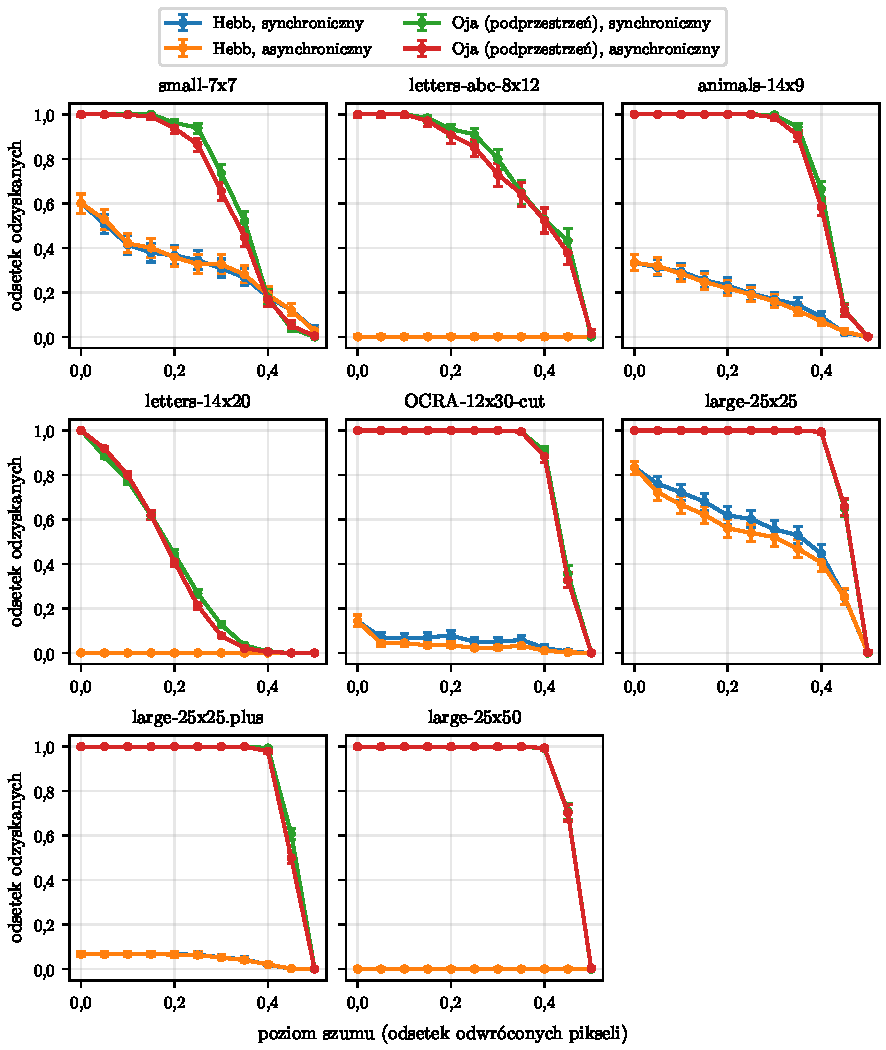
\includegraphics[width=0.75\textwidth]{noise/figures/recovery.pdf}
    \caption{Odsetek odzyskanych wzorców w zależności od poziomu szumu dla ośmiu dostarczonych zbiorów (100 prób na wzorzec, słupki to 95-procentowe przedziały Wilsona).}
    \label{fig:odzyskiwanie-szum}
\end{figure}

\noindent Reguła Oji odzyskuje prawie wszystkie wzorce do szumu od \num{0.35} do \num{0.4} w zbiorach o $N \ge 360$, a przy szumie \num{0.5} wejście jest średnio niezależne od celu i odzyskań prawie nie ma. Najmniejsze obszary przyciągania mają wzorce silnie skorelowanego zbioru \texttt{letters-14x20}. Błędy są tam jednak zwykle stanami najbliższymi celowi: poziom $f_{0,9}$ dla odsetka przebiegów kończących się najbliżej celu wynosi \num{0.2} (\num{0.15} w trybie asynchronicznym), a dla odzyskań 0 (\num{0.05}). Tryb asynchroniczny wypada przy dużym szumie zwykle nieco gorzej niż synchroniczny.

Poziomy krytyczne reguły Oji dla obu rodzajów uszkodzenia zebrano w Tabeli~\ref{tab:poziomy-krytyczne}. Zasłonięcie zmienia tylko czarne piksele pasa, więc przy tym samym poziomie zmienia mniej pikseli niż szum. Reguła Hebba traci przy nim odzyskania szybciej niż przy szumie, na przykład w \texttt{large-25x25} odsetek spada z \num{0.833} do \num{0.352} już przy poziomie \num{0.15}. Poziom zasłonięcia jest ułamkiem wysokości $H$ (rozdział~\ref{sec:uszkodzenia}), więc w \texttt{large-25x50} pas jest dwa razy wyższy niż w \texttt{large-25x25} i może zakryć także wspólną dolną połowę. Stąd niższe poziomy krytyczne tego zbioru przy zasłonięciu.

\begin{table}[H]
    \centering
    \caption{Poziomy krytyczne reguły Oji dla szumu i zasłonięcia. Gdy tryby się różnią, podano wartość dla trybu synchronicznego i asynchronicznego.}
    \label{tab:poziomy-krytyczne}
    \small
    \begin{tabular}{l c c c c}
        \toprule
        & \multicolumn{2}{c}{szum} & \multicolumn{2}{c}{zasłonięcie} \\
        \cmidrule(lr){2-3} \cmidrule(lr){4-5}
        Zbiór & $f_{0,9}$ & $f_{0,5}$ & $f_{0,9}$ & $f_{0,5}$ \\
        \midrule
        \texttt{small-7x7} & \num{0.25} / \num{0.2} & \num{0.35} / \num{0.3} & \num{0.3} & \num{0.6} \\
        \texttt{letters-abc-8x12} & \num{0.25} / \num{0.2} & \num{0.4} & \num{0.3} / \num{0.15} & \num{0.6} \\
        \texttt{animals-14x9} & \num{0.35} & \num{0.4} & \num{0.45} & \num{0.6} \\
        \texttt{letters-14x20} & 0 / \num{0.05} & \num{0.15} & 0 & \num{0.15} \\
        \texttt{OCRA-12x30-cut} & \num{0.4} / \num{0.35} & \num{0.4} & \num{0.3} & \num{0.6} / \num{0.45} \\
        \texttt{large-25x25} & \num{0.4} & \num{0.45} & \num{0.45} & \num{0.6} \\
        \texttt{large-25x25.plus} & \num{0.4} & \num{0.45} & \num{0.3} & \num{0.45} \\
        \texttt{large-25x50} & \num{0.4} & \num{0.45} & \num{0.15} & \num{0.3} \\
        \bottomrule
    \end{tabular}
\end{table}

\noindent Różnicę między regułami na jednym wejściu pokazuje Rysunek~\ref{fig:zasloniecie-przebieg}. Przy regule Hebba sieć kończy w stanie pozornym, który różni się od celu w 214 pikselach i jest najbliższy wzorcowi 3 ($m = \num{0.642}$).

\begin{figure}[H]
    \centering
    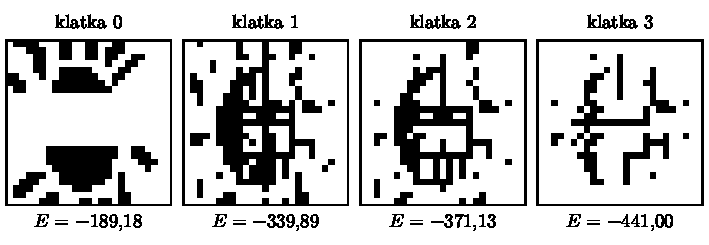
\includegraphics[width=0.8\textwidth]{occlusion/figures/recall-occlusion-hebb.pdf}

    \vspace{0.3cm}
    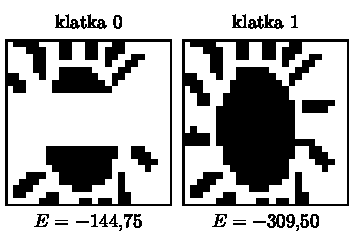
\includegraphics[width=0.4\textwidth]{occlusion/figures/recall-occlusion-oja.pdf}
    \caption{Odtwarzanie wzorca 0 zbioru \texttt{large-25x25} z wejścia z zasłoniętymi 8 wierszami (118 zmienionych pikseli, tryb synchroniczny, to samo wejście w klatce 0). Górny wykres: reguła Hebba. Dolny wykres: reguła Oji.}
    \label{fig:zasloniecie-przebieg}
\end{figure}

\subsection{Liczność zbioru}
\label{sec:odzyskiwanie-licznosc}

Wpływ liczby wzorców zbadano na początkowych fragmentach zbiorów \texttt{large-25x25.plus} i \texttt{letters-14x20}, przy stałym $N$ (Rysunek~\ref{fig:licznosc}). Przy regule Hebba odsetek odzyskań spada razem z liczbą stabilnych wzorców z rozdziału~\ref{sec:stabilnosc}. Dla liter sieć odzyskuje oba wzorce przy $p = 2$, a od $p = 5$ nie odzyskuje żadnego. Przy regule Oji obszar przyciągania obrazów kurczy się powoli. Odsetek odzyskań przy szumie \num{0.45} spada z \num{0.903} dla $p = 3$ do \num{0.608} dla $p = 15$, a poziom krytyczny $f_{0,9}$ wynosi \num{0.4} od $p = 6$ do $p = 15$. Dla liter kurczy się szybko, bo każda nowa litera jest silnie skorelowana z poprzednimi: $f_{0,9}$ spada z \num{0.35} przy $p = 2$ do 0 przy $p \ge 15$ (tryb synchroniczny). Liczność zbioru szkodzi więc niewiele, gdy wzorce są mało podobne, a bardzo, gdy są skorelowane.

\begin{figure}[H]
    \centering
    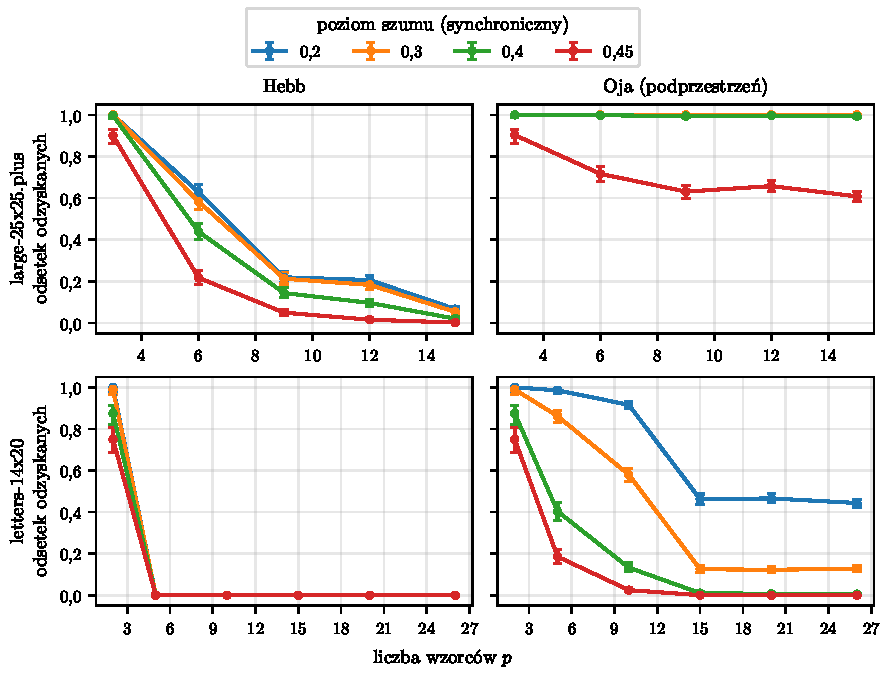
\includegraphics[width=0.65\textwidth]{load/figures/load.pdf}
    \caption{Odsetek odzyskanych wzorców w zależności od liczby wzorców $p$ dla początkowych fragmentów zbiorów \texttt{large-25x25.plus} (górne wykresy) i \texttt{letters-14x20} (dolne wykresy), dla czterech poziomów szumu w trybie synchronicznym. Lewa kolumna: reguła Hebba. Prawa kolumna: reguła Oji.}
    \label{fig:licznosc}
\end{figure}

\subsection{Grupy podobnych wzorców}
\label{sec:odzyskiwanie-grupy}

Zbiory grupowe (rozdział~\ref{sec:zbiory-dodatkowe}, Rysunek~\ref{fig:grupy}) mają po trzy grupy pięciu wariantów jednego obrazu, czyli $p = 15$ przy $N = 625$, tak jak zróżnicowany zbiór \texttt{large-25x25.plus}. Średnie nakładanie wariantów w grupie wynosi \num{0.920}, \num{0.815}, \num{0.639} i \num{0.361} dla $d = \num{0.02}$, \num{0.05}, \num{0.1} i \num{0.2}, a między grupami $\lvert m \rvert$ nie przekracza \num{0.155}. Wyniki pokazano na Rysunku~\ref{fig:odzyskiwanie-grupy}.

\begin{figure}[H]
    \centering
    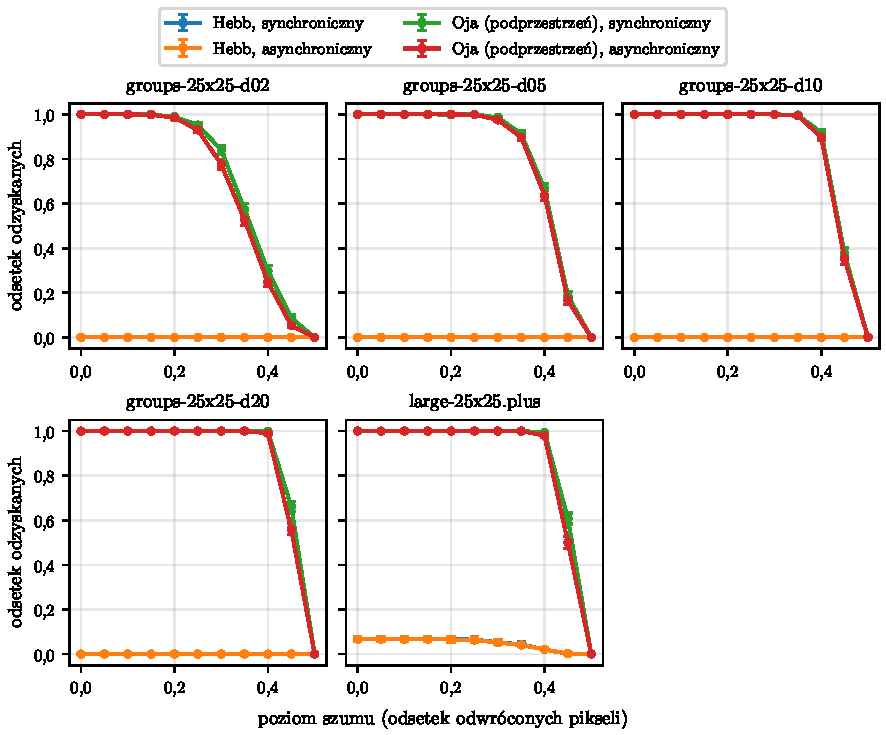
\includegraphics[width=0.65\textwidth]{groups/figures/recovery.pdf}
    \caption{Odsetek odzyskanych wzorców w zależności od poziomu szumu dla zbiorów grupowych i zróżnicowanego zbioru \texttt{large-25x25.plus} o tej samej liczności (100 prób na wzorzec). Linie reguły Hebba w trybach synchronicznym i asynchronicznym się pokrywają.}
    \label{fig:odzyskiwanie-grupy}
\end{figure}

\noindent Reguła Oji odzyskuje wszystkie warianty bez szumu, ale im bardziej są podobne, tym mniejszy obszar przyciągania ma każdy z nich. Poziom krytyczny $f_{0,9}$ rośnie z \num{0.25} dla $d = \num{0.02}$ do \num{0.4} dla $d = \num{0.2}$, czyli do wartości dla \texttt{large-25x25.plus}. Przy szumie \num{0.35} sieć odzyskuje \qty{57.4}{\percent} wariantów najbardziej podobnych grup, a w zbiorze zróżnicowanym wszystkie. Błędy zostają w grupie. Do szumu \num{0.4} przebieg kończy się we wzorcu innej grupy tylko w 2 przebiegach spośród wszystkich przebiegów zbiorów grupowych.

Reguła Hebba nie stabilizuje żadnego wariantu i zlewa każdą grupę w jeden stan, zgodnie z obserwacją Hopfielda o zlewaniu podobnych wzorców~\cite[s.~2557]{hopfield1982}. Przykład dla $d = \num{0.05}$ pokazano na Rysunku~\ref{fig:grupy-przebieg}. Wariant 0 podany bez szumu po jednym kroku przechodzi w stan równy w każdym pikselu większości pięciu wariantów grupy. Stan ten różni się od obrazu, z którego powstały warianty, tylko w 2 pikselach, a od samych wariantów w \numrange{29}{33} pikselach.

\begin{figure}[H]
    \centering
    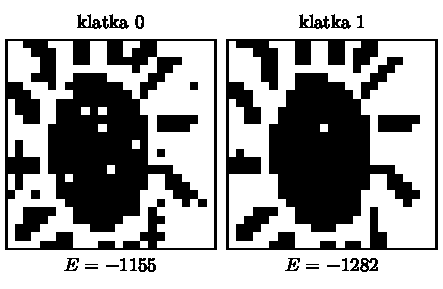
\includegraphics[width=0.5\textwidth]{groups/figures/recall-groups-hebb.pdf}
    \caption{Odtwarzanie wariantu 0 zbioru \texttt{groups-25x25-d05} bez szumu przy regule Hebba (tryb synchroniczny). Stan w klatce 1 to punkt stały.}
    \label{fig:grupy-przebieg}
\end{figure}
